 
%%%%%%%%%%%%% PREAMBLE %%%%%%%%%%%%%%%%%%%%%%%
\documentclass[a4paper, oneside]{book}


%%%%%%%%%%%%%%%%% PACKAGES %%%%%%%%%%%%%%%%%%%%
\usepackage[utf8]{inputenc}
\usepackage[T1]{fontenc}
%\usepackage{fontspec}
\usepackage{titlesec}
\usepackage{xcolor} % for black background white text
\titleformat{\chapter}[display]
  {\normalfont\bfseries\centering}{}{0pt}{\huge}  
\titlespacing*{\chapter}{0pt}{0pt}{10pt}

\usepackage[estonian]{babel}
\usepackage{gensymb}
\usepackage{graphicx}
\usepackage{pgfplots}
\usepackage{url}
\usepackage{cancel}
\usepackage{amsmath} % for \dfrac macro
\usepackage{subfig}
\usepackage[colorinlistoftodos]{todonotes}
\usepackage[colorlinks=true, allcolors=blue]{hyperref}
\usepackage{hyperref}
\usepackage{wrapfig} % to wrap text around figure
\newcommand\ddfrac[2]{{\displaystyle\frac{\displaystyle #1}{\displaystyle #2}}}


\usepackage{geometry} % LEHEKÜLJE GEOMEETRIA
 \geometry{
 a4paper,
 total={170mm,257mm},
 left=20mm,
 top=20mm,
 }


\usepackage{yfonts} % For gothic font

\usepackage[framemethod=tikz]{mdframed} % RUUDUSTIKU JAOKS

\usetikzlibrary{backgrounds}

\mdfdefinestyle{graphpaper}{%
    apptotikzsetting={\tikzset{mdfbackground/.style={}}},
    singleextra={%
        \scoped[on background layer,yshift=\mdfboundingboxheight]{\draw[step=5mm, line width=0.2mm, black!20!white] (0,0) grid (\mdfboundingboxwidth,-\mdfboundingboxheight);}
    },
}


\usepackage{titlepic} % For cover page
\usepackage{pdfpages}

\usepackage{tikz} % Igasuguste kujundite joonistamise jaoks
\usetikzlibrary{intersections, calc, angles} % nurkade joonestamise jaoks



%%%%%%%%%%%%%%%%%%%%%%%%%%%%%%%%%%%%%%%%%%%%%%%%%%%%%%%%%%%%%%%%%%%%%%%%%%%%%%%%%%%%%%
\usepackage{xparse,array} %korrutustabeli jaoks
\ExplSyntaxOn

\NewDocumentCommand{\multiplicationtable}{O{2em}m}
 {
  \azetina_multiplicationtable:nn { #1 } { #2 }
 }

\tl_new:N \l__azetina_multiplicationtable_tl

\cs_new_protected:Nn \azetina_multiplicationtable:nn
 {
  \tl_set:Nn \l__azetina_multiplicationtable_tl { $\times$ }
  \int_step_inline:nn { #2 }
   {
    \tl_put_right:Nn \l__azetina_multiplicationtable_tl { & ##1 }
   }
  \tl_put_right:Nn \l__azetina_multiplicationtable_tl { \\ \hline }
  \int_step_inline:nn { #2 }
   {
    \tl_put_right:Nn \l__azetina_multiplicationtable_tl { ##1 }
    \int_step_inline:nn { #2 }
     {
      \tl_put_right:Nx \l__azetina_multiplicationtable_tl
       {
        & \int_to_arabic:n { ##1*####1 }
       }
     }
    \tl_put_right:Nn \l__azetina_multiplicationtable_tl { \\ }
   }
  \begin{tabular}{ @{} r |@{}  *{#2}{w{r}{#1}@{}} }
  \tl_use:N \l__azetina_multiplicationtable_tl
  \end{tabular}
 }

\ExplSyntaxOff
%%%%%%%%%%%%%%%%%%%%%%%%%%%%%%%%%%%%%%%%%%%%%%%%%%%%%%%%%%%%%%%%%%%%%%%%%%%%%%%%%%%%%%%



% kaarte joonestamiseks:
\def\centerarc[#1](#2)(#3:#4:#5)% Syntax: [draw options] (center) (initial angle:final angle:radius)
    { \draw[#1] ($(#2)+({#5*cos(#3)},{#5*sin(#3)})$) arc (#3:#4:#5); }

\usepackage{tikz,tkz-euclide} % võrdsete haarade tähistamiseks

\usepackage{apacite} % tsiteeringute jaoks




%%%%%%%%%%% BEGINNING THE DOCUMENT %%%%%
\begin{document}

%%%%%%%%%%%%%%%% Tiitelleht %%%%%%%%%%%%%
\title{Füüsikaliste nähtuste modelleerimine}
\author{Artur Raag}
\date{2021}
\maketitle

%%%%% TOC järel ja pärast tühjad lehed %%%%%%%
\thispagestyle{empty}
\tableofcontents
\newpage
\thispagestyle{empty}

%\chapter{Sissejuhatus}
%\begin{flushleft}


Meie eesmärgiks on kujutada keha liikumist graafilisel tasapinnal. Kuna me kujutame liikumist tasapinnal, siis meil on keha asukoha määramiseks vaja kahte argumenti. Esimene neist peab meile ütlema keha horisontaalset asukohta (ehk kui vasakul või paremal ta asub), ning teine määrab vertikaalse asukoha (ehk kui kõrgel või madalal keha tasapinnal asub). 


Kasutame selle jaoks traditsioonilist Descartesi koordinaatsüsteemi.

\begin{figure}[h]  
\centering 
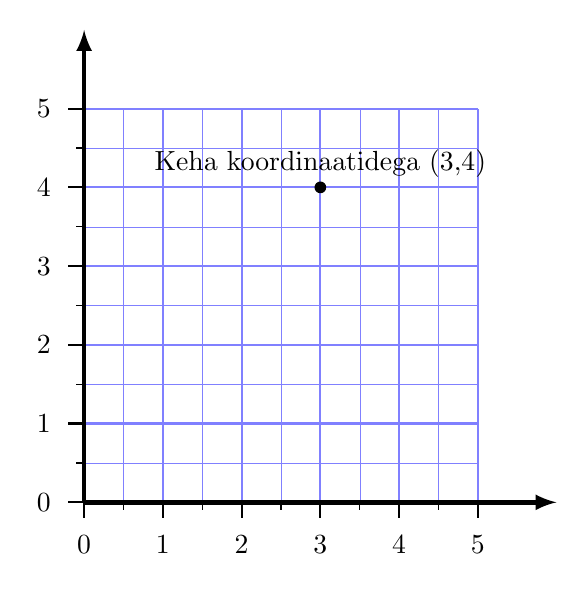
\begin{tikzpicture}
% Draw the grid
\tikzset{help lines/.style={color=blue!50}}
\draw[thick,step=1cm,help lines] (0,0) grid (5,5);
\draw[ultra thin,step=.5cm,help lines] (0,0) grid (5,5);
% Draw axes
\draw[ultra thick,-latex] (0,0) -- (6,0);
\draw[ultra thick,-latex] (0,0) -- (0,6);
% the co-ordinates -- major
\foreach \x in {0,1,...,5} {     % for x-axis
\draw [thick] (\x,0) -- (\x,-0.2);
}
\foreach \y in {0,1,...,5} {   %% for y-axis
\draw [thick] (0,\y) -- (-0.2,\y);
}
% the numbers
\foreach \x in {0,1,...,5} { \node [anchor=north] at (\x,-0.3) {\x}; }
\foreach \y in {0,1,...,5} { \node [anchor=east] at (-0.3,\y) {\y}; }
% the co-ordinates -- minor
\foreach \x in {.5,1.5,...,4.5} {
\draw [thin] (\x,0) -- (\x,-0.1);
}
\foreach \y in {.5,1.5,...,4.5} {
\draw [thin] (0,\y) -- (-0.1,\y);
}
\node at (3,4) [circle, fill, inner sep=1.5pt] {};
\node at (3,4)[anchor=south] {Keha koordinaatidega (3,4)};
\end{tikzpicture}
\caption{Keha asukoht tasapinnal}
\label{Joonis 1}
\end{figure}


Selline pilt kirjeldaks vaid ühte instantsi/iteratsiooni ehk ajahetke.
Selleks, et kujutada liikumist samal pinnal, tuleb meil joonist iga iteratsiooni/ajahetke järel uuendada.

Näiteks kui kujutada lineaarset liikumist, mis on määratud funktsiooniga $y=x+1$, kus $x$ määrabki ajahetke, ning keha algne asukoht on punktis $(1,2)$, siis saaksime järgmise kolme ajahetke jaoks kolm järgmist kaadrit:

\begin{figure}[h]  
\centering 

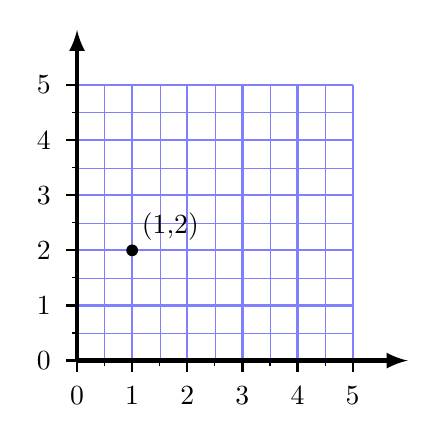
\begin{tikzpicture}[scale=0.7]
     % Draw the grid
\tikzset{help lines/.style={color=blue!50}}
\draw[thick,step=1cm,help lines] (0,0) grid (5,5);
\draw[ultra thin,step=.5cm,help lines] (0,0) grid (5,5);
% Draw axes
\draw[ultra thick,-latex] (0,0) -- (6,0);
\draw[ultra thick,-latex] (0,0) -- (0,6);
% the co-ordinates -- major
\foreach \x in {0,1,...,5} {     % for x-axis
\draw [thick] (\x,0) -- (\x,-0.2);
}
\foreach \y in {0,1,...,5} {   %% for y-axis
\draw [thick] (0,\y) -- (-0.2,\y);
}
% the numbers
\foreach \x in {0,1,...,5} { \node [anchor=north] at (\x,-0.3) {\x}; }
\foreach \y in {0,1,...,5} { \node [anchor=east] at (-0.3,\y) {\y}; }
% the co-ordinates -- minor
\foreach \x in {.5,1.5,...,4.5} {
\draw [thin] (\x,0) -- (\x,-0.1);
}
\foreach \y in {.5,1.5,...,4.5} {
\draw [thin] (0,\y) -- (-0.1,\y);
}
\node at (1,2) [circle, fill, inner sep=1.5pt] {};
\node at (1,2)[anchor=south west] {(1,2)};
\end{tikzpicture}% NO EMPTY LINE HERE!!!! 
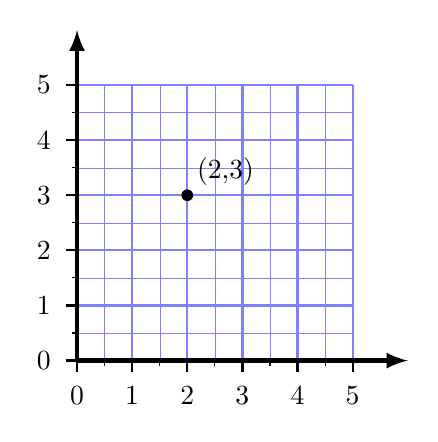
\begin{tikzpicture}[scale=0.7]  
     % Draw the grid
\tikzset{help lines/.style={color=blue!50}}
\draw[thick,step=1cm,help lines] (0,0) grid (5,5);
\draw[ultra thin,step=.5cm,help lines] (0,0) grid (5,5);
% Draw axes
\draw[ultra thick,-latex] (0,0) -- (6,0);
\draw[ultra thick,-latex] (0,0) -- (0,6);
% the co-ordinates -- major
\foreach \x in {0,1,...,5} {     % for x-axis
\draw [thick] (\x,0) -- (\x,-0.2);
}
\foreach \y in {0,1,...,5} {   %% for y-axis
\draw [thick] (0,\y) -- (-0.2,\y);
}
% the numbers
\foreach \x in {0,1,...,5} { \node [anchor=north] at (\x,-0.3) {\x}; }
\foreach \y in {0,1,...,5} { \node [anchor=east] at (-0.3,\y) {\y}; }
% the co-ordinates -- minor
\foreach \x in {.5,1.5,...,4.5} {
\draw [thin] (\x,0) -- (\x,-0.1);
}
\foreach \y in {.5,1.5,...,4.5} {
\draw [thin] (0,\y) -- (-0.1,\y);
}
\node at (2,3) [circle, fill, inner sep=1.5pt] {};
\node at (2,3)[anchor=south west] {(2,3)};
\end{tikzpicture}
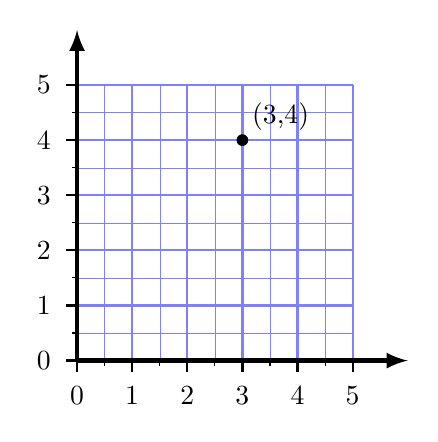
\begin{tikzpicture}[scale=0.7]
     % Draw the grid
\tikzset{help lines/.style={color=blue!50}}
\draw[thick,step=1cm,help lines] (0,0) grid (5,5);
\draw[ultra thin,step=.5cm,help lines] (0,0) grid (5,5);
% Draw axes
\draw[ultra thick,-latex] (0,0) -- (6,0);
\draw[ultra thick,-latex] (0,0) -- (0,6);
% the co-ordinates -- major
\foreach \x in {0,1,...,5} {     % for x-axis
\draw [thick] (\x,0) -- (\x,-0.2);
}
\foreach \y in {0,1,...,5} {   %% for y-axis
\draw [thick] (0,\y) -- (-0.2,\y);
}
% the numbers
\foreach \x in {0,1,...,5} { \node [anchor=north] at (\x,-0.3) {\x}; }
\foreach \y in {0,1,...,5} { \node [anchor=east] at (-0.3,\y) {\y}; }
% the co-ordinates -- minor
\foreach \x in {.5,1.5,...,4.5} {
\draw [thin] (\x,0) -- (\x,-0.1);
}
\foreach \y in {.5,1.5,...,4.5} {
\draw [thin] (0,\y) -- (-0.1,\y);
}
\node at (3,4) [circle, fill, inner sep=1.5pt] {};
\node at (3,4)[anchor=south west] {(3,4)};
\end{tikzpicture} 
\caption{Vasakul: Keha asukoht algsel ajahetkel. Keskel: Keha asukoht teisel ajahetkel. Paremal: Keha asukoht viimasel ajahetkel.} \label{Joonis 2}  
\end{figure}

Ehk vaatleja ekraanil näeks liikumine välja nagu (Joonis \ref{Joonis 3}).
\vspace{2mm}

\begin{figure}[h]
\centering
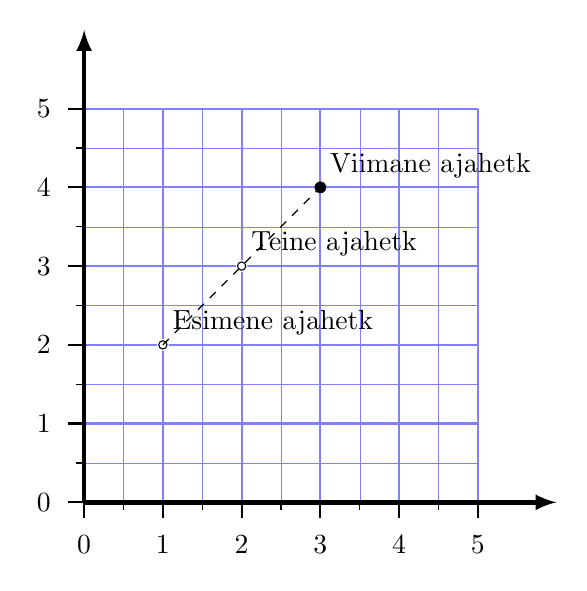
\begin{tikzpicture}
     % Draw the grid
\tikzset{help lines/.style={color=blue!50}}
\draw[thick,step=1cm,help lines] (0,0) grid (5,5);
\draw[ultra thin,step=.5cm,help lines] (0,0) grid (5,5);
% Draw axes
\draw[ultra thick,-latex] (0,0) -- (6,0);
\draw[ultra thick,-latex] (0,0) -- (0,6);
% the co-ordinates -- major
\foreach \x in {0,1,...,5} {     % for x-axis
\draw [thick] (\x,0) -- (\x,-0.2);
}
\foreach \y in {0,1,...,5} {   %% for y-axis
\draw [thick] (0,\y) -- (-0.2,\y);
}
% the numbers
\foreach \x in {0,1,...,5} { \node [anchor=north] at (\x,-0.3) {\x}; }
\foreach \y in {0,1,...,5} { \node [anchor=east] at (-0.3,\y) {\y}; }
% the co-ordinates -- minor
\foreach \x in {.5,1.5,...,4.5} {
\draw [thin] (\x,0) -- (\x,-0.1);
}
\foreach \y in {.5,1.5,...,4.5} {
\draw [thin] (0,\y) -- (-0.1,\y);
}
\node at (3,4) [circle, fill, inner sep=1.5pt] {};
\node at (3,4)[anchor=south west] {Viimane ajahetk};

\node at (2,3) [circle, fill=white, inner sep=1.5pt] {};
\node at (2,3)[anchor=south west] {Teine ajahetk};
\draw (2,3) circle (1.5pt);

\node at (1,2) [circle, fill=white, inner sep=1.5pt] {};
\node at (1,2)[anchor=south west] {Esimene ajahetk};
\draw (1,2) circle (1.5pt);
\draw[dashed] (1,2)--(3,4);
\end{tikzpicture}
\caption{Keha liikumine tasapinnal}
\label{Joonis 3}
\end{figure}

\vspace{2mm}
On näha, et keha justkui hüppaks punktist $(1,2)$ punkti $(2,3)$ ning viimaks ka punkti $(3,4)$. Ehk teisisõnu, see ei näe eriti liikumise moodi välja. Kahjuks ei saa reaalset liikumist ekraanil kujutada ning me peamegi piirduma selliste ''hüppetega'' punktist punkti. Küll aga on meil võimalus inimese silma natuke petta. Kui me vähendaksime ajahetkede vahemike, siis väheneksid ka ''hüppete'' vahemikud ja seega näeks liikumine märkimisväärselt sujuvam välja \cite{fpsyoutube}.

\vspace{2mm}
Kuid ajahetkede vahemike me lõputult väikseks teha ka ei saa, kuna sellisel juhul oleks arvuti sunnitud rohkem ja seega kauem arvutusi teostama.

\vspace{2mm}
Väidetavalt \cite{potter2014detecting} suudab inimese silm kujutist tuvastada 13 millisekundiga. Oma rakenduste loomisel, võikski sellise ajavahemikuga piirduda. Väiksema ajavahemiku valimine meie kujutise näivat liikumist ei täiustaks, kuna inimese silm ei jõuaks nii kui nii sellega järge pidada.

\vspace{2mm}
Meie rakenduste esimestel katsetel, proovime liikumisi arvutada 13 millisekundiliste ajahetkedega. Kui säärane ajavahemik osutub arvuti jaoks ülejõu käivaks, siis suurendame ajahetkede vahemike sammuga 13, seni kuni saavutame piisavalt sobiva tulemuse.


\end{flushleft}

\chapter{Kepleri teooria}
\begin{flushleft}


Selleks, et modelleerida keha liikumist ümber valitud taevakeha, tuleb meil leida:

\begin{itemize}
\item kuidas keha koordinaadid $x(t)$ ja $y(t)$ sõltuvad ajast. 


\item kuidas kiirusvektori projektsioonid $v_{x}(t)$ ja $v_{y}(t)$ sõltuvad ajast.

\item millised on keha kineetilised, potentsiaalsed ja kogu energiad erinevatel ajahetkedel?
\end{itemize}

Sellejaoks tuleb meil kirja panna liikumisvõrrand, mille saame Newtoni teise seaduse kaudu:

\begin{equation}
\label{eq1}
\vec{F}=m\vec{a}
\end{equation}

Kui me eeldame, et sateliit kehale mõjub vaid gravitatsiooni jõud, siis saame asendada $F$-i hoopis $F_{g}$-ga:

\begin{equation}
\label{eq2}
\vec{F_{g}}= -G \cdot \dfrac{m \cdot M}{r^{3}}\cdot \vec{r}
\end{equation}

Siinkohal tasub mainida, et potentsiaalse energia valem on [\textbf{\textcolor{red}{TÕESTA!!!!!!!!!!!}}]:

\begin{equation}
\label{eq3}
U_{pot}=-G\cdot \dfrac{m \cdot M}{r}
\end{equation}

Siin valemites on $G$ gravitatsiooni konstant, $M$ on Maa mass, $m$ sateliidi mass ning $r$ on kahe keha tsentrite vaheline kaugus. Viimast suurust saab ümber kirjutada ka kujul $r=R_{M}+h$, kus $R_{M}$ on keha keskmine raadius ning $h$ on sateliidi kõrgus maapinna suhtes.

Asendades $F_{g}$ valemisse (\ref{eq1}), saame:

\begin{equation}
\label{eq4}
-G \cdot \dfrac{m \cdot M}{r^{3}}\cdot \vec{r} = m \vec{a}
\end{equation}

Jagame mõlemad võrduse pooled $m$-iga ning saame

\begin{equation}
\label{eq5}
\vec{a}=-G \cdot \dfrac{M}{r^{3}}\cdot \vec{r} 
\end{equation}

Jaotame vektori $x$ ja $y$ komponentideks. Teame, et asukoha teist järku tuletis, annab meile kiirenduse, ning esimest järku tuletis annab meile kiiruse. Seega:



\begin{equation}
\label{eq6}
\begin{cases}
\ddot{x}=-G \cdot \dfrac{M}{r^{3}}\cdot x\\
\ddot{y}=-G \cdot \dfrac{M}{r^{3}}\cdot y
\end{cases}
\end{equation}

, kusjuures

\begin{equation}
\label{eq7}
r= \sqrt{x^{2}+y^{2}}
\end{equation}

Asendades $v_{x}=\dot{x}$, $a_{x}=\dot{v_{x}}=\ddot{x}$ ning $v_{y}=\dot{y}$, $a_{y}=\dot{v_{y}}=\ddot{y}$, saame me kahe teistjärku differentsiaalvõrrandite süsteemi asemel hoopis esimest järku nelja võrrandisüsteemi.


\begin{equation}
\label{eq8}
\begin{cases}
\dot{x}=v_{x}\\
\dot{y}=v_{y}\\
\dot{v_{x}}=-G\dfrac{M}{r^{3}}\cdot x\\
\dot{v_{y}}=-G\dfrac{M}{r^{3}}\cdot y

\end{cases}
\end{equation}

Diferentsiaalvõrrandite süsteemi lahendamiseks kasutame rkf45 algorütmi.

Samuti on näha, et võrrandisüsteemi lahendamiseks on vaja määrata algkiirused $v_{x}$ ja $v_{y}$ ning algkoordinaadid $x$ ja $y$.

\textbf{\textcolor{red}{Siin jääb võrrandisüsteemini jõudmine ikkagi veidi häguseks/müstikaks. Ilmselt peaks enne seda uurima mida RKF45 täpsemalt teeb, seda siin kirjeldama ja sellest tegema ka järelduse millist võrrandisüsteemi me lõpuks soovime. UURI JAAN JANNO ÕPIKUT LK 196}}

\subsection{Ühikute teisendamine}

Kuna meil on peamiselt tegemist makrokehadega, mille kiirused on hästi suured, siis tasuks nende kiirused teisendada meeter/sekundilt kilomeeter/sekundiks.

\vspace{2mm}
Ehk kui esialgu on kiirus ühikuga $m/s$, siis selle teisendamisel $km/s$-ks tuleb meil kiirust laiendada $1000$-ga. Suuruse laiendamine meil tegelikult midagi ei muuda, kuna $1000$-ed taanduksid ära. Põhjus miks me aga seda teeme, on sellepärast, et kiirus, mis on esialgu $m/s$, muutuks $1000$-ga läbi jagades $km/s$-ks, mis oleks omakorda veel läbi korrutatud $1000$-ga. Ehk teisisõnu, kiiruste või kauguste teisendamisel meetrilt kilomeetrile, tuleb meil suurus lihtsalt $1000$-ga läbi korrutada.

\vspace{5mm}
Ehk matemaatiliselt: $v_{x}\left[\dfrac{m}{s} \right]=\dfrac{1000 \cdot v_{x}[m/s]}{1000}\longrightarrow \left[ \begin{tabular}{c}
$v_{x}/1000$ \\
on kiirus km/s.
\end{tabular} \right] \longrightarrow 1000 \cdot v_{x} \left[\dfrac{km}{s} \right]$

\vspace{5mm}
Seega võrrandite
\[ 
\begin{cases}
\dot{x}=v_{x}\\
\dot{y}=v_{y}
\end{cases}
\]
puhul, tuleb meil mõlemad võrduse pooled korrutada 1000-ga.

\vspace{5mm}
Saame:
\begin{equation}
\begin{cases}
1000 \cdot \dot{x}=1000 \cdot v_{x}\\
1000 \cdot \dot{y} = 1000 \cdot v_{y}
\end{cases}
\longrightarrow 
\begin{cases}
\dot{x}=v_{x}\\
\dot{y}=v_{y}
\end{cases}
\end{equation} 

Mõlemalt võrduse poolelt taanduvad $1000$-d ära, mis tähendab seda, et võime vabalt esimesed kaks võrrandit teisendada meeter/sekundilt kilomeeter/sekundiks kasutamata igasuguseid koefitsente.

\vspace{5mm}
Võrrandite 
\[
\begin{cases}
\dot{v_{x}}=-G\dfrac{M}{r^{3}}\cdot x\\
\dot{v_{y}}=-G\dfrac{M}{r^{3}}\cdot y

\end{cases}\]
puhul analoogselt käitudes saame:

\vspace{5mm}

\begin{equation}
\begin{cases}
1000 \cdot \dot{v_{x}}=-G\dfrac{M}{(10^{3} \cdot r)^{3}}\cdot 1000 \cdot x\\
1000 \cdot \dot{v_{y}}=-G\dfrac{M}{(10^{3} \cdot r)^{3}}\cdot 1000 \cdot y
\end{cases}
\longrightarrow
\begin{cases}
\dot{v_{x}}=-G\dfrac{M}{10^{9} \cdot r^{3}} \cdot x\\
\dot{v_{y}}=-G\dfrac{M}{10^{9} \cdot r^{3}} \cdot y
\end{cases}
\longrightarrow
\begin{cases}
\dot{v_{x}}=-G\dfrac{M \cdot 10^{-9}}{r^{3}}\cdot x\\
\dot{v_{y}}=-G\dfrac{M \cdot 10^{-9}}{r^{3}}\cdot y
\end{cases}
\end{equation}

Ehk kiirenduste puhul tuleb meil eduka teisenduse jaoks korrutada võrrandite paremad pooled koefitsendiga $10^{-9}$.

\end{flushleft}


\chapter{Lend kuule teooria}
\begin{flushleft}
Kui sateliit piisavalt kaugele Maa atmosfäärist liigub, siis võiks arvestada ka teiste taevakehade gravitatsiooniväljadega. Praegusel juhul piirdume enda mudelis vaid Maa ja Kuu gravitatsioonijõuga. Taustsüsteemiks valime Maa.

\vspace{5mm}
Mitme kehale mõjuva jõu(vektori) puhul tuleb jõud(vektorid) lihtsalt lineaarselt kokku liita. Seda tasub eriti silmas pidada juhul, kui me kavatseme tulevikus kehale muid mõjuvaid jõudusid arvesse võtta.

\vspace{5mm}
Sateliidile mõjuvad jõud on järgmised:

\begin{equation}
\label{eq3_1}
F_{Maa}=-G\dfrac{m \cdot M_{m}}{r_{m}^{3}}\cdot \vec{r_{m}}
\end{equation}

\begin{equation}
\label{eq3_2}
F_{Kuu}=-G\dfrac{m \cdot M_{k}}{r_{k}^{3}}\cdot \vec{r_{k}}
\end{equation}


Kus $F_{Maa}$ ja $F_{Kuu}$ on vastavate taevakehade poolt tekitatud gravitatsioonijõud, $M_{m}$ ja $M_{k}$ vastavate taevakehade massid, $r_{m}$ ja $r_{k}$ vastavate taevakehade tsentrite ja satteliidi kaugused, $m$ sateliidi mass ning $G$ gravitatsiooni konstant.


\vspace{5mm}
\subsection{Esimene kosmiline kiirus}

\vspace{5mm}
Tasub meeles pidada, et kui meie esialgne kiirus ei ole piisavalt suur, siis langeb meie sateliit Maa peale tagasi. Vähimat kiirust, mida sateliit saavutama peab, selleks et jääda ringjoonelisele orbiidile, nimetatakse \textbf{esimeseks kosmiliseks kiiruseks}.

\vspace{5mm}
Kui eeldada, et keha liigub ringjooneliselt mööda Maa pinda, siis saaksime keha liikumise kirjeldamiseks järgmise liikumis võrrandi: 

\begin{equation}
\label{eq3_3}
 m \cdot a =F=m\cdot g
\end{equation}
kus $g$ on raskuskiirendus Maa pinna lähedal.

Keha, mille omapäraks on ringjooneline liikumine, saab kirjeldada ka tsentrifugaal jõu kaudu:

\begin{equation}
\label{eq3_4}
F_{c}=\dfrac{mv^{2}}{R_{Maa}}
\end{equation}

Pannes valemid \ref{eq3_3} ja \ref{eq3_4} üksteisega võrduma, saame avaldada keha vähima kiiruse, mis on tarvis ringjooneliseks orbiidiks Maa pinna lähedal.

\begin{equation}
\label{eq3_5}
\dfrac{mv^{2}}{R_{Maa}} = mg \longrightarrow v = \sqrt{\dfrac{\cancel{m}gR_{Maa}}{\cancel{m}}} \longrightarrow v= \sqrt{gR_{Maa}}
\end{equation}

Kuid ideaalis on orbiidis olev keha ikkagi Maa pinnast veidi eemal. Selle jaoks tuleb meil valemit \ref{eq3_5} veidi täiendada.

Esmalt paneme kirja uuesti üldise liikumisvõrrandi:

\begin{equation}
\label{eq3_6}
ma=F=-G\dfrac{m \cdot M_{Maa}}{r^{2}}
\end{equation}

, kusjuures

\begin{equation}
\label{eq3_7}
r=R_{Maa}+h
\end{equation}

Tsentrifugaaljõudu tuleb samuti üldistada, kuna see võib samuti kõrgusest sõltuda. Seega:

\begin{equation}
\label{eq3_8}
F_{c}=\dfrac{mv^{2}}{(R_{Maa}+h)}
\end{equation}

Paneme valemid \ref{eq3_6} ja \ref{eq3_7} üksteisega võrduma 

\begin{equation}
\label{eq3_9}
-G\dfrac{m \cdot M_{Maa}}{(R_{Maa}+h)^{2}} = \dfrac{mv^{2}}{(R_{Maa}+h)}
\end{equation}

ning tuletan sellest viimaks vähima kiiruse, mis on vajalik antud kõrgusel Maa pinnast, ringjoonelise orbiidi säilitamiseks:

\begin{equation}
\label{eq3_10}
v_{I}= \sqrt{\dfrac{G\cancel{m}M_{Maa}\cancel{(R_{Maa}+h)}}{\cancel{m}\cancel{(R_{Maa} + h)^{2}}}} = \sqrt{\dfrac{GM_{Maa}}{(R_{Maa}+h)}}
\end{equation}

\textcolor{red}{Miinusmärk?}

Valemi \ref{eq3_10} eeskirja järgi võime öelda, et kui keha kõrgusel $h$ liigub aeglasemini kui kiirusega $v_{I}$, siis langeb antud keha tagasi Maa peale.

\vspace{5mm}
\subsection{Teine kosmiline kiirus}

\vspace{5mm}
Kui me soovime leida vähimat kiirust, mis on vajalik keha jaoks, et lennata Maa mõjusfäärist välja (lõpmatusse), siis saame seda arvutada kasutades energiajäävuse seadust:

\begin{equation}
\label{eq3_11}
E_{tot}= E_{pot} + E_{kin}
\end{equation}

Kus $E_{tot}$, $E_{pot}$ ja $E_{kin}$ on kogueneriga, potentsiaalne energia ning kineetiline energia.

Kahe keha vahelist potentsiaalset energiat saab arvutada valemiga:

\begin{equation}
\label{eq3_12}
E_{pot} = - \dfrac{G\cdot m \cdot M}{R}
\end{equation}

Ning kineetilist energiat valemiga:

\begin{equation}
\label{eq3_13}
E_{kin} = \dfrac{mv^{2}}{2}
\end{equation}

\vspace{5mm}
Seega keha kogu energia maa pinnalt õhku tõustes on

\begin{equation}
\label{eq3_14}
E_{0}= - \dfrac{G\cdot m \cdot M}{R} + \dfrac{mv_{II}^{2}}{2}
\end{equation}

, kus $v_{II}$ on vähim kiirus, et Maa mõjusfäärist välja lennata.

\vspace{5mm}
Lõpmata kaugel, peaks keha koguenergia võrduma nulliga, ehk

\begin{equation}
\label{eq3_15}
E_{1}= 0
\end{equation}

Energia jäävuse seaduse tõttu, peab energia alghetkel olema sama, mis viimasel hetkel, ehk nad peavad olema võrdsed. Seega:

\begin{equation}
\label{eq3_16}
E_{0} = E_{1} \longrightarrow - \dfrac{G\cdot m \cdot M}{R} + \dfrac{mv_{II}^{2}}{2} = 0
\end{equation}

Avaldades $v_{II}$ me saame:

\begin{equation}
\label{eq3_17}
v_{II}=\sqrt{\dfrac{2GmM}{Rm}} \longrightarrow v_{II}=\sqrt{\dfrac{2GM}{R}}
\end{equation}

\vspace{5mm}
\subsection{Liikumisvõrrand}

\vspace{5mm}
Kuna meie kehale mõjub jõud nii Maa kui ka Kuu poolt, siis tuleb meil liikumisvõrrand need kaks jõudu kokku liita.

\begin{equation}
\label{eq3_18}
F= m \cdot \vec{a} \longrightarrow -G\dfrac{m \cdot M_{m}}{r_{m}^{3}}\cdot \vec{r} - G \dfrac{m \cdot M_{k}}{|\vec{R}-\vec{r_{m}}|^{3}}\cdot(\vec{R}-\vec{r_{m}}) = m\cdot \vec{a}
\end{equation}

Jagame mõlemad võrduse pooled $m$-iga

\begin{equation}
\label{eq3_19}
-G\dfrac{\cancel{m} \cdot M_{m}}{r_{m}^{3}}\cdot \vec{r} - G \dfrac{\cancel{m} \cdot M_{k}}{|\vec{R}-\vec{r_{m}}|^{3}}\cdot(\vec{R}-\vec{r_{m}}) = \cancel{m}\cdot \vec{a}
\end{equation}

Järele jääb

\begin{equation}
\label{eq3_20}
-G\dfrac{ M_{m}}{r_{m}^{3}}\cdot \vec{r} - G \dfrac{ M_{k}}{|\vec{R}-\vec{r_{m}}|^{3}}\cdot(\vec{R}-\vec{r_{m}}) = \vec{a}
\end{equation}

Teisendades kõik vektorid $x$ ja $y$ komponentideks ning arvestades, et $v_{x}=\dot{x}$, $a_{x}=\dot{v_{x}}=\ddot{x}$ ning $v_{y}=\dot{y}$, $a_{y}=\dot{v_{y}}=\ddot{y}$, saame me kahe teistjärku differentsiaalvõrrandite süsteemi asemel hoopis esimest järku nelja võrrandisüsteemi.

\begin{equation}
\label{eq3_21}
\begin{cases}
\dot{x}=v_{x}\\
\dot{y} = v_{y}\\
\ddot{x} = - \dfrac{G \cdot M_{m} \cdot 10^{-9}}{(x_{m}^{2}+y_{m}^{2})^{3/2}}\cdot x_{m} - \dfrac{G \cdot M_{k} \cdot 10^{-9}}{((X-x_{m})^{2}+(Y-y_{m})^{2})^{3/2}}\cdot (X-x_{m}) \\
\ddot{y} = - \dfrac{G \cdot M_{m} \cdot 10^{-9}}{(x_{m}^{2}+y_{m}^{2})^{3/2}}\cdot y_{m} - \dfrac{G \cdot M_{k} \cdot 10^{-9}}{((X-x_{m})^{2}+(Y-y_{m})^{2})^{3/2}} \cdot (Y-y_{m})

\end{cases}
\end{equation}

Saime võrrandisüsteemi, mis kirjeldab sateliidi liikumist  tasapinnal. Meie taustsüsteem/koordinaadistik on fikseeritud Maa keskpunktis kuid modeleerime kahe taevakeha (Maa ja Kuu) ning ühe sateliidi liikumist. Sateliidi jaoks on võrrandisüsteem olemas \ref{eq3_21}, kuid Kuu liikumise kirjeldamiseks meil veel midagi ei ole.

\vspace{5mm}
Kuna taustsüsteem on fikseeritud Maaga ja hetkel eeldame, et Kuu tiirleb ümber Maakera ringjooneliselt pideva kiirusega $v_{kuu}\approx 1.022$ $km/s$, siis Kuu liikumist saab kirjeldada järgmise võrrandisüsteemiga:

\begin{equation}
\label{eq3_22}
\begin{cases}
X_{kuu}=R\cdot cos(\omega \cdot t)\\
Y_{kuu} = R \cdot sin(\omega \cdot t)
\end{cases}
\end{equation}

kus $R$ kaugus Maa ja Kuu vahel, $t$ on aeg, $\omega$ on Kuu nurkkiirus, kusjuures

\begin{equation}
\label{eq3_23}
\omega=\dfrac{v_{kuu}}{R} = \dfrac{2 \cdot \pi}{T}
\end{equation}

Võrrandeid \ref{eq3_22} diferentseerima ei pea, kuna nad sõltuvad ainult ajast.
\end{flushleft}

\chapter{Runge-Kutta Fehlberg meetod}

\begin{flushleft}

Meie mudelites/simulatsioonides esineb erinevaid diferentsiaalvõrrandeid, mille lahendamiseks kasutame 4ndat järku Runge Kutta Fehlberg meetodit.

\section{RKF meetodi kirjeldus}

Meetodi edukaks rakendamiseks on vaja määrata ära algtingimus:

\begin{equation}
y'=f(x,y) \hspace{5mm} y(x_{0})=y_{0}
\end{equation}

ning kuna meetod on iteratiivne, siis tuleb määrata ära ka (integreerimise)samm $h$ ($x$-i järgi). Diferentsiaalvõrrandi funktsiooni väärtust järgmises punktis arvutatakse järgmise eeskirja järgi:

\begin{equation}
y_{n+1}=y_{n}+\dfrac{h}{6}\cdot(k_{1}+2k_{2}+2k_{3}+k_{4}),
\end{equation}
kus 

\begin{equation}
k_{1}=f(x_{n},y_{n})
\end{equation}

\begin{equation}
k_{2}=f(x_{n}+\dfrac{h}{2},y_{n}+\dfrac{h}{2}k_{1})
\end{equation}

\begin{equation}
k_{3}=f(x_{n}+\dfrac{h}{2},y_{n}+\dfrac{h}{2}k_{2})
\end{equation}

\begin{equation}
k_{4}=f(x_{n}+h,y_{n}+hk_{3})
\end{equation}


\section{RKF45}
Hetkel eeldasime, et samm $h$ on fikseeritud, kuid see võib meie lahenduse täpsust vähendada. Täpsema tulemuse saamiseks kasutame optimiseeritud Runge Kutta Fehlberg meetodit (RKF45), millel on adaptiivsed omadused. 

Nimelt leitakse differentsiaalvõrrandi kaks ligikaudset lahendit, mida seejärel võrreldakse. Kui lahendid on oma väärtuste poolest piisavalt sarnased, siis võetakse lahend vastu ja minnakse üle järgmisele iteratsioonile. Kui lahendite täpsus on määratud täpsusest madalam, siis (integreerimis)sammu $h$ vähendatakse. Analoogselt kui lahendite täpsus on määratud täpsusest suurem, siis (integreerimis)sammu $h$ suurendatakse ning tehakse kogu iteratsioon uuesti uue sammuga läbi enne järgmisele iteratsioonile asumist.

Ka arvutamise eeskiri erineb veidi eelnevalt mainitud RKF meetodist.

\begin{equation}
\begin{split}
&k_{1}=h \cdot f(x+A(1) \cdot h, y) \\
&k_{2}=h \cdot f(x+A(2)\cdot h, y+B(2,1) \cdot k_{1})\\
&k_{3}=h \cdot f(x+A(3)\cdot h, y+B(3,1)\cdot k_{1} + B(3,2) \cdot k_{2})\\
&k_{4}=h \cdot f(x+A(4)\cdot h, y+B(4,1)\cdot k_{1} + B(4,2) \cdot k_{2} + B(4,3)\cdot k_{3})\\
&k_{5}=h \cdot f(x+A(5)\cdot h, y+B(5,1)\cdot k_{1} + B(5,2) \cdot k_{2} + B(5,3)\cdot k_{3} + B(5,4)\cdot k_{4})\\
&k_{6}=h \cdot f(x+A(6)\cdot h, y+B(6,1)\cdot k_{1} + B(6,2) \cdot k_{2} + B(6,3)\cdot k_{3} + B(6,4)\cdot k_{4}+B(6,5)\cdot k_{5}),\\
\end{split}
\label{RKF45_K}
\end{equation}

kus $A(k)$ ning $B(k,l)$ on Fehlbergi poolt tuletatud koefitsendid, ning on leitavad tabelist \ref{table_1}.


\begin{table}[h]
\centering
\begin{tabular}{|c|c|c|c|c|c|c|c|c|}
\hline
k&A(k)&B(k,1)&B(k,2)&B(k,3)&B(k,4)&B(k,5)&CH(k)&CT(k)\\
\hline
1&0&0&0&0&0&0&16/135&1/360\\
\hline
2&1/4&1/4&0&0&0&0&0&0\\
\hline
3&3/8&3/32 & 9/32 & 0 & 0 & 0& 6656/12825 & -128/4275 \\
\hline
4&12/13&1932/2197 & -7200/2197 & 7296/2197 & 0 & 0 & 28561/56430 & -2197/75240\\
\hline
5&1&439/216 & -8 & 3680/513 & -845/4104 & 0& -9/50&1/50\\
\hline
6&1/2&-8/27 & 2 & -3544/2565 & 1859/4104 & -11/40& 2/55 & 2/55 \\
\hline
\end{tabular}
\caption{ $A$ ja $B$ koefitsendid}
\label{table_1}
\end{table}

Diferentsiaalvõrrandi lahend leitakse nõnda:

\begin{equation}
y_{n+1}=y_{n}+CH(1)\cdot k_{1}+CH(2)\cdot k_{2}+CH(3)\cdot k_{3}+CH(4)\cdot k_{4}+CH(5)\cdot k_{5}+CH(6)\cdot k_{6}
\end{equation}

ning kärpimisviga, millega määrame ära kas muudame enda sammu või mitte, arvutatakse:

\begin{equation}
TE=|CT(1)\cdot k_{1}+CT(2)\cdot k_{2}+CT(3) \cdot k_{3}+CT(4) \cdot k_{4} + CT(5) \cdot k_{5}+CT(6) \cdot k_{6}|,
\end{equation}

kus $CT(k)$ ning $CH(k)$ on samuti Fehlbergi poolt tuletatud koefitsendid ning leitavad tabelist \ref{table_1}.

Kui viga $TE> \epsilon$ ($\epsilon$ - meie poolt määratud täpsus) , siis asendame eelmise sammu $h$ uue sammuga $h_{uus}$ ning kordame iteratsiooni. Kui $TE \leq \epsilon$, siis saame jätkata järgmist iteratsiooni ning asendame sammu $h$ uue sammuga $h_{uus}$.

Uut sammu arvutame valemiga:

\begin{equation}
h_{uus}=0.9 \cdot h \cdot \left( \dfrac{\epsilon}{TE}\right)^{1/5}
\end{equation}

\end{flushleft}


\chapter{RKF45 realiseerimine programmeerimis keeltes P5JS näitel}
\begin{flushleft}

\section{Fehlbergi koefitsendid}
 
Selleks, et tabelis \ref{table_1} määratud koefitsentidele lihtsamini ligi pääseda, oleks mõistlik koefitsendid kirjutada andmemassiividena/maatriksitena. Nendele pääseb ligi indekseid kasutades.


Ehk:

\begin{equation}
A(k)=
\begin{pmatrix}
0\\
1/4\\
3/8\\
12/13\\
1\\
1/2
\end{pmatrix}
\end{equation}
 

\begin{equation}
B(k,l)=
\begin{pmatrix}
0&0&0&0&0\\

1/4&0&0&0&0\\

3/32 & 9/32 & 0 & 0 & 0 \\

1932/2197 & -7200/2197 & 7296/2197 & 0 & 0\\

439/216 & -8 & 3680/513 & -845/4104 & 0\\

-8/27 & 2 & -3544/2565 & 1859/4104 & -11/40 \\
\end{pmatrix}
\end{equation}

\begin{equation}
CH(k)=
\begin{pmatrix}
16/135\\
0\\
6656/12825\\
28561/56430\\
-9/50\\
2/55
\end{pmatrix}
\hspace{10mm}
CT(k)=
\begin{pmatrix}
1/360\\
0\\
-128/4275\\
-2197/75240\\
1/50\\
2/55
\end{pmatrix}
\end{equation}


Ka tõusudest $k_{i}$ loome massiivi:

\begin{equation}
k_{i}=
\begin{pmatrix}
k_{1}\\
k_{2}\\
k_{3}\\
k_{4}\\
k_{5}\\
k_{6}
\end{pmatrix}
\end{equation}  

Kuid meie mudelites esineb diferentsiaalvõrrandeid, mida lahendada soovime, rohkem kui üks. Seega, iga differentsiaalvõrrandi kohta, mida lahendame, tuleb lisada veel üks veerg $k$-sid. Ehk üldisemalt

\begin{equation}
k_{i,n}=
\begin{pmatrix}
k_{1,1} & k_{1,2} & ...& k_{1,n} \\
k_{2,1}& k_{2,2} & ...& k_{2,n}\\
k_{3,1}& k_{3,2} & ...& k_{3,n}\\
k_{4,1}& k_{4,2} & ...& k_{4,n}\\
k_{5,1}& k_{5,2} & ...& k_{5,n}\\
k_{6,1}& k_{6,2} & ...& k_{6,n}
\end{pmatrix}
\end{equation}  

kus $i$ on koefitsendi järjekorranumber(?) ja $n$ on võrrandi järjekorranumber.

Programmeerimiskeeles P5JS alustatakse iteratsioonide loendamist arvust 0, mitte 1, mida tasub ka programmi realiseerimisel meeles pidada.

\end{flushleft}

\chapter{Lennard-Jonesi potentsiaal}
\begin{flushleft}

\section{Lennard-Jones potentsiaal}
 
Lennard-Jonesi potentsiaal on defineeritud järgnevalt
\begin{equation} \label{eq_5.1}
V(r)=4 \epsilon \left[ \left( \dfrac{\sigma}{r} \right)^{12}- \left( \dfrac{\sigma}{r} \right)^{6} \right]
\end{equation}
kus $V$ on potentsiaal, $r$ on osakeste vaheline kaugus.

Osakeste vahelise kauguse $r$ moodul on defineeritud kui

\begin{equation} \label{eq_5.2}
%r=\overrightarrow{r_{i,j}}=\overrightarrow{r_{j}}-\overrightarrow{r_{i}}
r_{i,j}=\sqrt{(x_{j}-x_{i})^{2}+(y_{j}-y_{i})^{2}}
\end{equation}

kus $x_{j}$ ja $y_{j}$ on esimese ning $x_{i}$ ja $y_{i}$ on teise osakese asukoha vektori koordinaadid.

Kui rakendada $ \nabla $ operaatorit Lennard-Jonesi potentsiaalile \ref{eq_5.1}, siis saaksime jõu kahe osakese vahel, mis näeb välja nõnda:

\begin{equation} \label{eq_5.3}
\vec{F}=-\nabla V
\end{equation}

kus $V$ on Lennard-Jonesi potentsiaal \ref{eq_5.1}, ning

\begin{equation} \label{eq_5.4}
\nabla =\left[ \dfrac{ \delta }{\delta x} \hat{i}+\dfrac{\delta}{\delta y} \hat{j} \right]
\end{equation}



\begin{center}
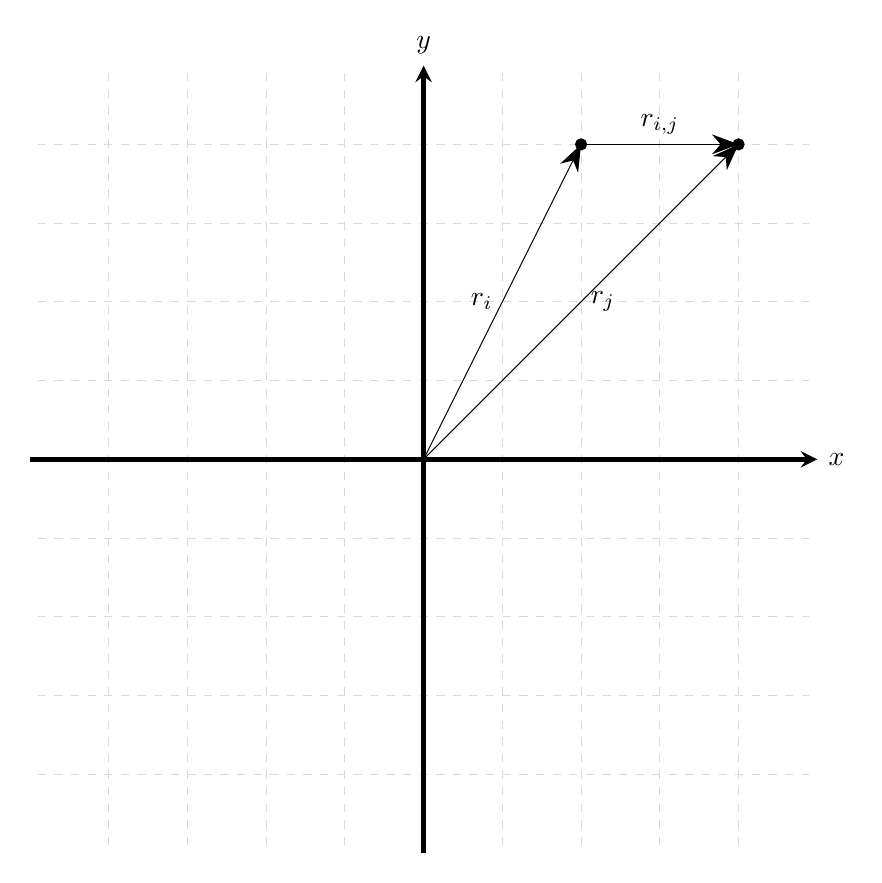
\begin{tikzpicture}
\draw[help lines, color=gray!30, dashed] (-4.9,-4.9) grid (4.9,4.9);
\draw[-stealth,ultra thick] (-5,0)--(5,0) node[right]{$x$};
\draw[-stealth,ultra thick] (0,-5)--(0,5) node[above]{$y$};
\draw[-{Stealth[scale=2]}] (0,0)--(2,4) node[midway,left]{$r_{i}$};
\draw[-{Stealth[scale=2]}](0,0)--(4,4) node[midway,right]{$r_{j}$};
\filldraw[black] (2,4) circle (2pt);
\filldraw[black] (4,4) circle (2pt);
\draw[-{Stealth[scale=2]}](2,4)--(4,4) node [midway, above] {$r_{i,j}$};
\end{tikzpicture}
\end{center}

\textbf{Valemi tuletus KATSE 1:}



\[F=-4 \epsilon \left[ \sigma^{12} \dfrac{\delta}{\delta x} \left( r^{-12} \right) \hat{i}-\sigma^{6} \dfrac{\delta}{\delta x} (r^{-6}) \hat{i}+\sigma^{12} \dfrac{\delta}{\delta y} (r^{-12}) \hat{j} -\sigma^{6} \dfrac{\delta}{\delta y} (r^{-6}) \hat{j}\right]=... \]

Olgu $r$ hoopis $ r=\sqrt{x^{2}+y^{2}} $. Sellisel juhul tuleb

\[...= -4 \epsilon \left[ \sigma^{12} \dfrac{\delta}{\delta x} (x^{2}+y^{2})^{-6} \hat{i}-\sigma^{6} \dfrac{\delta}{\delta x} (x^{2}+y^{2})^{-3} \hat{i}+\sigma^{12} \dfrac{\delta}{\delta y} (x^{2}+y^{2})^{-6} \hat{j} -\sigma^{6} \dfrac{\delta}{\delta y} (x^{2}+y^{2})^{-3} \hat{j}\right]=...\]

Tuletiste arvutamisel võtame, et $(x^{2}+y^{2})=u$ (Chain Rule). Seega tuleb arvutada tuletised 
\[\dfrac{\delta}{\delta u} (u^{-6}) \cdot \dfrac{\delta}{\delta x} (x^{2}+y^{2}) \]

\[\dfrac{\delta}{\delta u} (u^{-6}) \cdot \dfrac{\delta}{\delta y} (x^{2}+y^{2}) \]

\[\dfrac{\delta}{\delta u} (u^{-3}) \cdot \dfrac{\delta}{\delta x} (x^{2}+y^{2}) \]

\[\dfrac{\delta}{\delta u} (u^{-3}) \cdot \dfrac{\delta}{\delta y} (x^{2}+y^{2}) \]

Need välja arvutades saame jätkata jõu valemi tuletamist

\[...=-4 \epsilon \left( \left[-12x \sigma^{12}(x^{2}+y^{2})^{-7}-6x \sigma^{6}(x^{2}+y^{2})^{-4} \right] \hat{i}+ \left[-12y \sigma^{12}(x^{2}+y^{2})^{-7}-6y \sigma^{6}(x^{2}+y^{2})^{-4} \right] \hat{j} \right) =...\]

\[...=-4 \epsilon \left(6x \sigma^{6} \left[-2 \sigma^{6}(x^{2}+y^{2})^{-7}- (x^{2}+y^{2})^{-4} \right] \hat{i}+6y \sigma^{6} \left[-2 \sigma^{6}(x^{2}+y^{2})^{-7}-(x^{2}+y^{2})^{-4} \right] \hat{j} \right) =...\]


\[...=-24  \epsilon \sigma^{6} \left(x  \left[-2 \sigma^{6}(x^{2}+y^{2})^{-7}- (x^{2}+y^{2})^{-4} \right] \hat{i}+y \left[-2 \sigma^{6}(x^{2}+y^{2})^{-7}-(x^{2}+y^{2})^{-4} \right] \hat{j} \right)  \]

Ehk:

\begin{equation} \label{eq_5.5}
F_{x}=-24 \epsilon \sigma^{6} x \left[ -2 \sigma^{6}(x^{2}+y^{2})^{-7}-(x^{2}+y^{2})^{-4} \right]
\end{equation}

\begin{equation} \label{eq_5.6}
F_{y}=-24 \epsilon \sigma^{6} y \left[ -2 \sigma^{6}(x^{2}+y^{2})^{-7}-(x^{2}+y^{2})^{-4} \right]
\end{equation}

\textbf{Valemi tuletus KATSE 2:}

\begin{equation} \label{eq_5.7}
\nabla V(r)=4 \epsilon \left[ \dfrac{\delta V}{\delta x_{i} }\hat{i}+\dfrac{\delta V}{\delta y_{i}}\hat{j} \right]
\end{equation}

\begin{equation}
V(r)=4 \epsilon \left[ \sigma^{12} r^{-12}-\sigma^{6} \cdot r^{-6} \right]
\end{equation}


\begin{equation} \label{eq_5.8}
\nabla V(r)=4 \epsilon \nabla \left[ \sigma^{12} \left[(x_{i}-x_{j})\hat{i} + (y_{i}-y_{j}) \hat{j} \right]^{-12} -\sigma^{6} \left[ (x_{i}-x_{j})\hat{i} +(y_{i}-y_{j})\hat{j} \right]^{-6} \right]
\end{equation}

Asendan vektoriaalse $r$ hoopis modulaarse $r$-iga, kuna jõud kahe osakese vahel suunast ei sõltu, sõltub vaid moodulist: $r=\sqrt{(x_{i}-x_{j})^{2}+(y_{i}-y_{j})^{2}}$.

\begin{equation} \label{eq_5.9}
\nabla V(r)=4 \epsilon \nabla \left[ \sigma^{12} \left[(x_{i}-x_{j})^{2}+(y_{i}-y_{j})^{2} \right]^{-6} -\sigma^{6} \left[ (x_{i}-x_{j})^{2}+(y_{i}-y_{j})^{2} \right]^{-3} \right]
\end{equation}


Tuleb arvutada järgmised osatuletised:

\begin{equation} \label{eq_5.11}
 \dfrac{\delta }{\delta x_{i}} \underbrace{((x_{i}-x_{j})^{2}+(y_{i}-y_{j})^{2})^{-6}}_{u} \cdot \hat{i}=\dfrac{\delta}{\delta u} (u)^{-6} \cdot  \dfrac{\delta }{\delta x_{i}} \left( (x_{i}-x_{j})^{2}+\cancel{(y_{i}-y_{j})^{2}} \right)\cdot \hat{i}
\end{equation}

Teised tuletised analoogselt...

\begin{equation} \label{eq_5.12}
\dfrac{\delta }{\delta y_{i}}((x_{i}-x_{j})^{2}+(y_{i}-y_{j})^{2})^{-6} \cdot \hat{j}
\end{equation}

\begin{equation} \label{eq_5.13}
 \dfrac{\delta }{\delta x_{i}}((x_{i}-x_{j})^{2}+(y_{i}-y_{j})^{2})^{-3} \cdot \hat{i}
\end{equation}

\begin{equation} \label{eq_5.14}
 \dfrac{\delta }{\delta y_{i}}((x_{i}-x_{j})^{2}+(y_{i}-y_{j})^{2})^{-3}\cdot \hat{j} 
\end{equation}

Alustame osatuletisega \ref{eq_5.11}

\[ \dfrac{\delta }{\delta x_{i}} \underbrace{((x_{i}-x_{j})^{2}+(y_{i}-y_{j})^{2})^{-6}}_{u}\cdot \hat{i} =\dfrac{\delta}{\delta u} (u)^{-6} \cdot  \dfrac{\delta }{\delta x_{i}} \left( (x_{i}-x_{j})^{2}+\cancel{(y_{i}-y_{j})^{2}} \right) \cdot \hat{i}=\]

\[= -6((x_{i}-x_{j})^{2}+(y_{i}-y_{j})^{2}) ^{-7} \cdot \dfrac{\delta}{\delta x_{i}} (\underbrace{x_{i}-x_{j}}_{v})^{2} \cdot \hat{i}=\]

\[ = -6 \cdot \left(  (x_{i} -x_{j})^{2}+(y_{i}-y_{j})^{2}\right)^{-7} \cdot \dfrac{\delta}{\delta v} (v)^{2} \cdot \dfrac{\delta}{\delta x_{i}}(x_{i}-x_{j}) \cdot \hat{i}= \]

\[=-6 \cdot \left(  (x_{i} -x_{j})^{2}+(y_{i}-y_{j})^{2}\right)^{-7} \cdot 2 (x_{i}-x_{j}) \cdot 1 \cdot \hat{i} =\]

\[=-12 \cdot \left(  (x_{i} -x_{j})^{2}+(y_{i}-y_{j})^{2}\right)^{-7} \cdot  (x_{i}-x_{j}) \cdot \hat{i} \]

Jätame \ref{eq_5.12} esialgu vahele, vaatleme hoopis \ref{eq_5.13}, siis saame jõu $F_{x}$.

\[ \dfrac{\delta }{\delta x_{i}}((x_{i}-x_{j})^{2}+(y_{i}-y_{j})^{2})^{-3} \cdot \hat{i}= -3((x_{i}-x_{j})^{2}+(y_{i}-y_{j})^{2}) ^{-4} \cdot \dfrac{\delta}{\delta x_{i}} (\underbrace{x_{i}-x_{j}}_{v})^{2} \cdot \hat{i}=\]

\[=-3((x_{i}-x_{j})^{2}+(y_{i}-y_{j})^{2}) ^{-4} \cdot 2 (x_{i}-x_{j}) \hat{i}= \]

\[=-6((x_{i}-x_{j})^{2}+(y_{i}-y_{j})^{2}) ^{-4} \cdot (x_{i}-x_{j}) \hat{i} \]

Kui panna viimased kaks tulemust kokku, siis saame, et $F_{x}$:

\[
F_{x}=4 \epsilon \sigma^{6} (12 \sigma^{6} \cdot \left(  (x_{i} -x_{j})^{2}+(y_{i}-y_{j})^{2}\right)^{-7} \cdot  (x_{i}+x_{j}) \cdot \hat{i}  -6((x_{i}-x_{j})^{2}+(y_{i}-y_{j})^{2}) ^{-4} \cdot (x_{i}-x_{j}) \hat{i})
\]

Kui veidi lihtsustada...

\begin{equation} \label{eq_5.15}
F_{x}=24 \epsilon \sigma^{6} [2\sigma^{6}((x_{i} -x_{j})^{2}+(y_{i}-y_{j})^{2})^{-7}-((x_{i}-x_{j})^{2}+(y_{i}-y_{j})^{2}) ^{-4}] \cdot (x_{i}-x_{j}) 
\end{equation}

Analoogselt $F_{y}$-i tuletisi \ref{eq_5.12} ja \ref{eq_5.14} arvutades saame:

\begin{equation} \label{eq_5.16}
F_{y}=24 \epsilon \sigma^{6} [2\sigma^{6}((x_{i} -x_{j})^{2}+(y_{i}-y_{j})^{2})^{-7}-((x_{i}-x_{j})^{2}+(y_{i}-y_{j})^{2}) ^{-4}] \cdot (y_{i}-y_{j})
\end{equation}

\section{Kiirendus}

Kui asendada valemid \ref{eq_5.15} ja \ref{eq_5.16} Newtoni II seadusesse, siis saaksime avaldada kiirendused.

\begin{equation} \label{eq_5.17}
F=ma
\end{equation}

\begin{equation} \label{eq_5.18}
24 \epsilon \sigma^{6} [2\sigma^{6}((x_{i} -x_{j})^{2}+(y_{i}-y_{j})^{2})^{-7}-((x_{i}-x_{j})^{2}+(y_{i}-y_{j})^{2}) ^{-4}] \cdot (x_{i}-x_{j})=ma
\end{equation}

Jagame mõlemad võrduse pooled miga

\begin{equation} \label{eq_5.19}
a_{x}=\dfrac{24 \epsilon \sigma^{6} [2\sigma^{6}((x_{i} -x_{j})^{2}+(y_{i}-y_{j})^{2})^{-7}-((x_{i}-x_{j})^{2}+(y_{i}-y_{j})^{2}) ^{-4}] \cdot (x_{i}-x_{j})}{m}

\end{equation}

\end{flushleft}

\pagebreak
%\bibliographystyle{apacite}
%\bibliography{References}

\end{document}